\documentclass{article}
\usepackage{tikz}
\usepackage{caption}

\begin{document}

Lorem ipsum dolor sit amet, consectetuer adipiscing elit. Ut purus elit, vestibulum ut, placerat ac, adipiscing vitae, felis.

\begin{figure}[h]
    \centering
    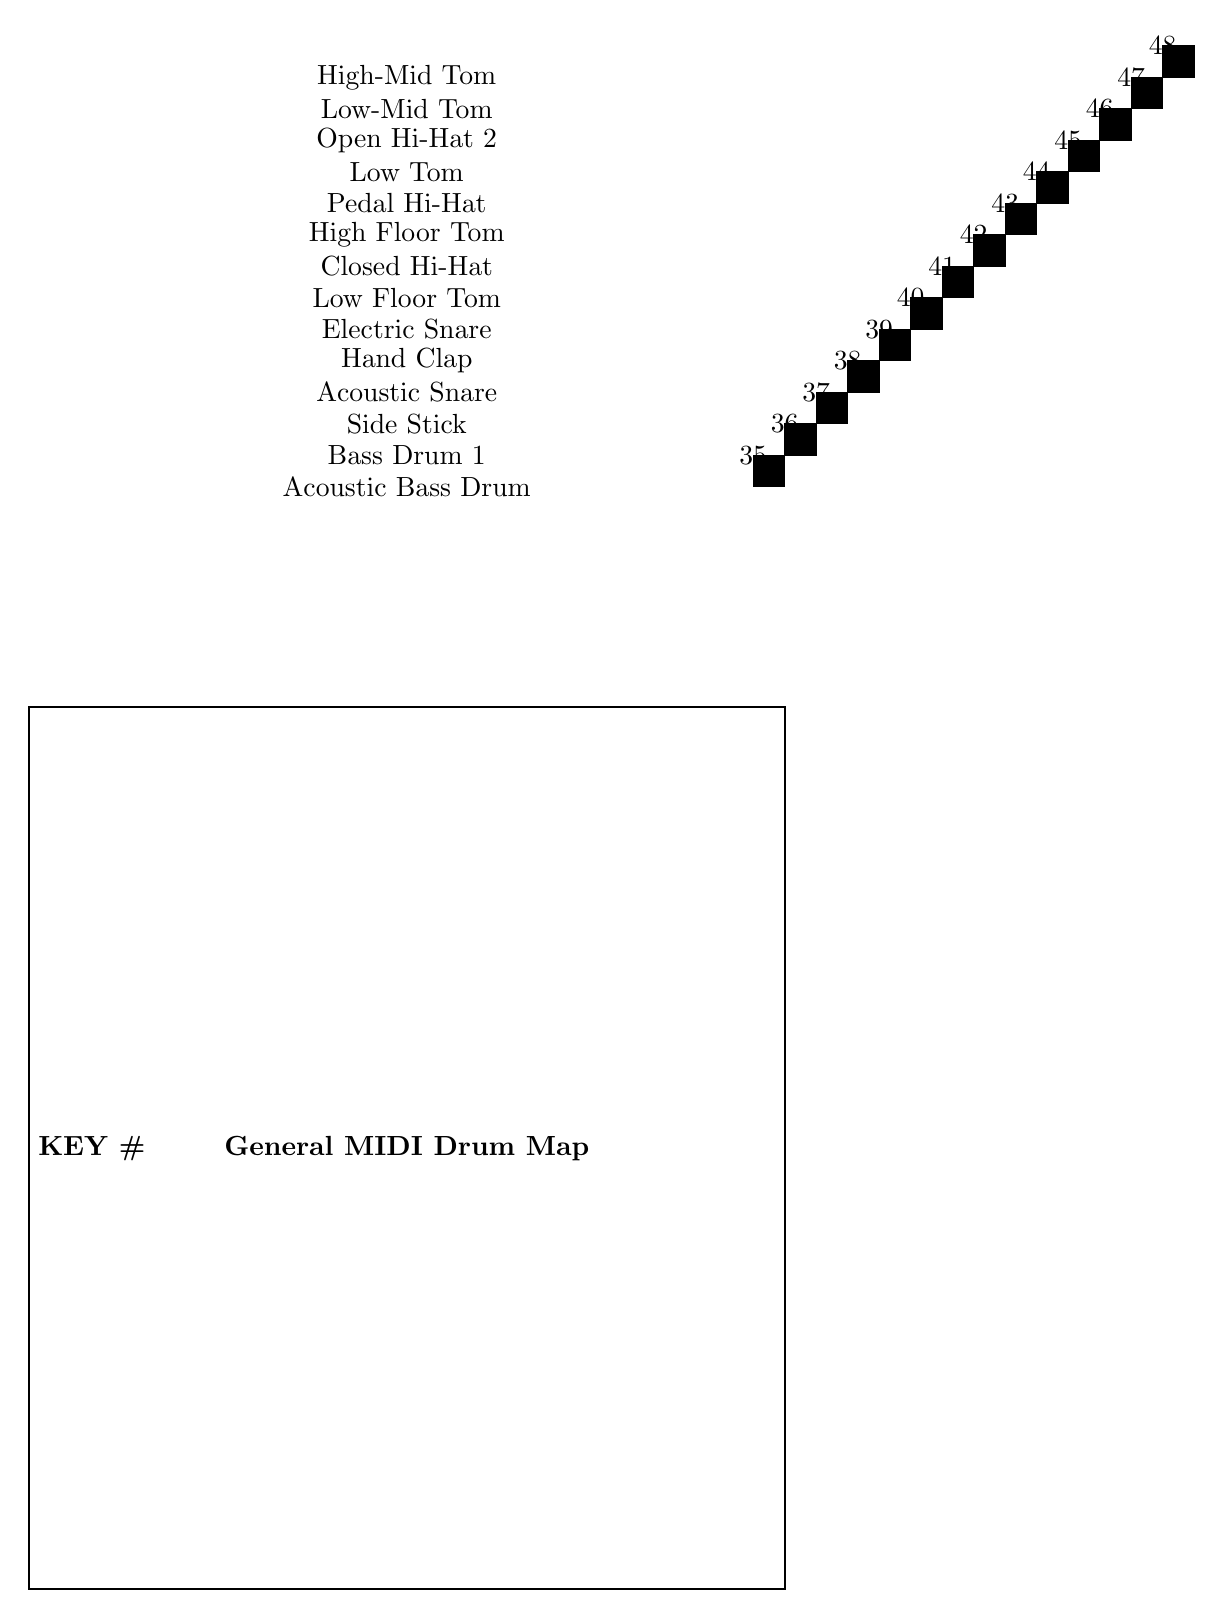
\begin{tikzpicture}[scale=0.8]
        % Table header
        \draw[thick] (0,0) rectangle (12,14);
        \node at (6,7) {\textbf{General MIDI Drum Map}};
        \node at (1,7) {\textbf{KEY \#}};
        
        % Key numbers
        \foreach \x in {35,...,48} {
            \draw[fill=black] (\x*0.5-6, 0.5*\x) rectangle ++(0.5, 0.5);
            \node at (\x*0.5-6, 0.5*\x+0.5) {\x};
        }
        
        % Drum names
        \node at (6, 0.5*35) {Acoustic Bass Drum};
        \node at (6, 0.5*36) {Bass Drum 1};
        \node at (6, 0.5*37) {Side Stick};
        \node at (6, 0.5*38) {Acoustic Snare};
        \node at (6, 0.5*39) {Hand Clap};
        \node at (6, 0.5*40) {Electric Snare};
        \node at (6, 0.5*41) {Low Floor Tom};
        \node at (6, 0.5*42) {Closed Hi-Hat};
        \node at (6, 0.5*43) {High Floor Tom};
        \node at (6, 0.5*44) {Pedal Hi-Hat};
        \node at (6, 0.5*45) {Low Tom};
        \node at (6, 0.5*46) {Open Hi-Hat 2};
        \node at (6, 0.5*47) {Low-Mid Tom};
        \node at (6, 0.5*48) {High-Mid Tom};
    \end{tikzpicture}
    
    \caption{General MIDI Drum Map}
    \label{fig:general_midi_drum_map}
\end{figure}

Nam dui ligula, fringilla a, euismod sodales, sollicitudin vel, wisi. Morbi auctor lorem non justo. Nam lacus libero, pretium at, lobortis vitae, ultricies et, tellus. Donec aliquet, tortor sed accumsan bibendum, erat ligula aliquet magna, vitae ornare odio metus a mi. Morbi ac orci et nisl hendrerit mollis. Suspendisse ut massa. Cras nec ante. Pellentesque a nulla. Cum sociis natoque penatibus et magnis dis parturient montes, nascetur ridiculus mus. Aliquam tincidunt urna. Nulla ullamcorper vestibulum turpis. Pellentesque cursus luctus mauris.
\end{document}